\subsection{Objectives}
\label{sub:objectives}
\smallskip

As outlined in part B1, this proposal is composed of 5 interconnected work packages. 
The proposal’s overarching aim is to discover or constrain the particle nature of dark matter via its production at the LHC and the contextualization of these results in the global DM theoretical and experimental landscape. 
The basis for reaching this aim is the implementation of data-taking techniques that enable the ATLAS experiment to obtain a much bigger physics output from the upcoming LHC dataset without requiring a significant increase in resources. 
Physics results and software tools resulting this proposal will be shared with the broader DM community. 


The main objectives of the \textsc{Realdark} WPs are: 

\begin{description}

%In \textsc{Realdark} we will use novel data taking techniques (developed in Work Package 1) to \textbf{further the systematic exploration} of the hadronic decays of the DM mediator as in the left-hand side of Fig.~\ref{fig:feynman} (WP2-3). 

\item[(WP1)]  \textbf{To extend the capabilities of the ATLAS trigger system} with a comprehensive set of real-time analysis techniques. 
%The first cornerstone of WP1 are the TLA technique and the Partial Event Building (PEB) technique, which overcomes the traditional paradigm of first recording all detector data and then analyzing it by performing the data analysis directly at the trigger level, so that the majority of raw detector data can be dropped. 
In WP1, we will:
\begin{enumerate} 
\item implement photons, electrons and muons in TLA, starting from the jet prototype developed in my StG;
\item contribute to a suite of reconstruction and calibration techniques for HLT objects that can also be used offline;
\item implement a combination of PEB and TLA techniques targeting complex detector signatures;
\item study ML data compression techniques to be used for TLA data and beyond in future LHC runs. 
\end{enumerate}
%We will also seek further gains in storage using machine learning algorithms for data compression. %this sentence makes no sense
\item[(WP2)] \textbf{To commission the upgraded ATLAS trigger with early Run-3 data}, using searches that already have a solid methodological basis from Run-2. In WP2 we will:
\begin{enumerate} 
\item study the performance of physics objects reconstructed and calibrated at the HLT and offline; 
\item deploy and validate new calibrations and real-time analysis techniques with well-established generic searches for new phenomena in the dijet spectrum;
\item prepare end-to-end analysis code to be used for faster analysis turnaround and as part of the dissemination strategy.  
% such as generic high- and low-mass dijet (TLA). 
\end{enumerate} 
%We will deploy  for new phenomena that can already lead to groundbreaking results in the earlier stages of LHC data taking. The outcomes of this WP will be physics results with a the new LHC data, as well as tools and publications measuring the performance of trigger and offline objects.  

\item[(WP3-WP4)] To use the LHC dataset recorded with novel data taking techniques to perform searches sensitive to two broad classes of DM models:
 
\begin{itemize} 
\item in WP3, we will search for hadronic decays of WIMP DM mediators in the dijet and dijet+ISR final states using a TLA that including both photons and jets, to probe electroweak-scale mediator masses not fully explored by traditional searches.
\item in WP4, we will search for dark matter candidates and dark photons within the jets as predicted from dark QCD, using a combination of TLA and PEB to recover sensitivity to signals that escape traditional detector reconstruction techniques.
\end{itemize}

\item[(WP5)] \textbf{To disseminate and communicate physics results and tools} to make them possible to the broader DM and experimental community. In WP5 we will: 

\begin{enumerate} 
\item collaborate with theory experts to identify the most promising parameter space for searches in WP4. 
\item contribute to organizing and leading the new cross-community initiative for DM that I co-founded in 2019 (\href{https://indico.cern.ch/e/iDMEu/}{iDMEu}), including nuclear physics, astroparticle physics and particle physics.
\item disseminate technical outcomes of WP1 to other experiments at the LHC and beyond. 
\item disseminate the outcome of the searches in WP3 and WP4, whether they are a discovery to be characterized or constraints that will guide future DM experiments. The latter two objectives will be supported by my role in the \href{https://hepsoftwarefoundation.org}{HEP Software Foundation} and by my involvement in the \href{https://projectescape.eu}{ESCAPE project}, as detailed below. 
\end{enumerate} 

\end{description}

The objectives of each WP are developed in more detail in the following sections, with intermediate objectives and milestones marked with \textbf{[N]} matching Sec.~\ref{sec:ProjectPlanning}.

% and their interconnections are displayed in \textbf{Fig.~\ref{fig:WPs}}. 

\subsubsection{Objectives of WP1}

The first objective of WP1 is to \textbf{deploy a comprensive TLA stream in ATLAS within the new multithreaded ATLAS HLT software}. %mentioned above?
In Run-3, this project will allow offline-quality photons, muons and electrons to be used for physics analysis, in addition to jets. 
The success of the jet prototype has been demonstrated in Run-2 within my StG. 
The use of a jet TLA allowed to lower the HLT jet threshold from 420 GeV in traditional analysis to 220 GeV in TLA, bringing orders-of-magnitude improvements in the number of recorded events. 
A TLA implementation of HLT photons (\textbf{[1]}) will bring significant improvements to the sensitivity of the dijet+ISR DM mediator search. 
The HLT analyzes all photon and electron candidates that have a $p_{\rm{T}}$ above 30 GeV, 
while only single-photon events with a $p_{\rm{T}}$ above 150 GeV are retained in traditional analysis. 
The work done and lessons learned in the case of trigger-level jets will be the stepping stone for adding photons to the TLA stream, 
and doubling the signal acceptance for the dijet+ISR search. 
The implementation of electrons (\textbf{[2]}) and muons (\textbf{[3]}) in TLA will follow that of photons.
% but they will not be a priority for first data as the difference in thresholds between online and offline events is limited. 
While electron and muon TLAs can still bring significant improvement to e.g. dark photon searches below the Z peak~\cite{ToBeCited}, %CMSDimuon
the aim of this work is to gain confidence with the challenges of reconstruction and calibration of different physics objects with constrained computing resources. 

As a second objective of WP1, we will \textbf{develop the calibration techniques that are necessary to enable physics analysis} with a reduced HLT-level data format, achieving near-parity with offline performance. 
With my StG team, I have been responsible for reaching a 1-permille agreement in the jet energy scale of trigger-level jets~\cite{ToBeCited}.%TLAPRL 
Within \textsc{Realdark} we will ensure that this is still the case for jets as our main observables, as well as for other physics objects. 
In particular, the performance of trigger-level photons obtained in Run-2~\cite{ToBeCited} %EGamma paper
and preliminary studies performed by a Lund Bachelor’s student~\cite{ToBeCited}%LeoBachelorThesis
already give sufficient confidence on the feasibility of a dijet+ISR search, where the resonance is built from the jets and the photon is used as a tag. 
The main challenge for this search lies in distinguishing low-$p_{\rm{T}}$ hard-scatter jets from pile-up jets, and efficiently subtracting pile-up contributions. 
In WP1, we will test new pile-up suppression and subtraction techniques using calorimeter information and the newly available tracking information. 

The third objective of WP1 is to \textbf{implement and reconstruct a data stream combining physics objects reconstructed at the trigger level and selected raw information in restricted regions of the detector}, through the combination of the TLA and Partial Event Building (PEB) techniques \textbf{[4]}. 
Deployed for the first time in ATLAS in this proposal, this combination will maintain a sufficiently small data format with an amount of information equivalent to traditional techniques. 
It will be a necessary ingredient to enable the non-standard reconstructions needed for the searches in WP4, and enable further characterization of potential excesses in a TLA search. 
The overall outcome of this work will be a technical publication detailing the early Run-3 trigger \textbf{[5]}.  

Preliminary estimates based on the Run-2 $B-$physics PEB %cite muon paper if available
place the size of TLA+PEB events to less than half of a standard event. 
To remain advantageous, TLA and PEB must have the minimal possible footprint in terms of both storage and computing power. 
Joint work betwen WP1 and WP2-4 will ensure that these constraints are met with dedicated trigger selections and selections.   
The budget of this proposal also includes storage servers that will be used to store this data in 2023-2024. 

The fourth objective of WP1 is to \textbf{further reduce the storage load of TLA events (and more generally ATLAS data and simulation) by compressing this data}. 
TLA data is ideally suited for studies of more aggressive (lossy) compression, since it has already been shown that it can be made robust against loss of information using dedicated calibrations. If compression and decompression algorithms are sufficiently fast (order of milliseconds) they do not significantly increase the amount of resources needed for data processing. 
The use of machine learning techniques for fast and performant compression (e.g. of images) is widespread: inspired by this, my ATLAS collaborators and I have been supervising Lund University Master’s students in preliminary tests to compress TLA data using deep autoencoders~\cite{ToBeCited}. %cite autoencoders paper 
When compressing 2017 TLA jet data, these studies demonstrated that a compression of factor better than 2 can be achieved with a negligible performance loss.  
In this proposal we plan to continue this work and deploy this compression algorithm in a proof-of-principle yet realistic emulation of the trigger system using raw detector data \textbf{[7]}. This is a future-looking study targeting HL-LHC, but if the results are ready to be deployed during the course of Run-3 we will use them for compression of the data recorded with techniques in WP1. Work will be documented in technical publications \textbf{[6,8]}.
%Is this also ok with TLA+PEB? 

As the trigger system is crucial for this research program and for the overall ATLAS physics output, the Lund group will maintain a leading role in its operations. 
Throughout the course of this project, the team members will be involved in the development and monitoring of trigger software. 
This is a particularly crucial responsibility during the run up to first data taking, after the complete overhaul of the ATLAS software. 
The Lund group has already taken responsibility roles in the trigger, with the StG postdoc William Kalderon (now a postdoctoral fellow at BNL), who has served for two years as the convenor of the jet trigger and has now moved on to be overall ATLAS trigger menu coordinator. 

\subsubsection{Objectives of WP2}

The overall objective of WP2 is the commissioning of the new trigger techniques using data at the LHC start-up, and their validation using well-established physics observables. These observables will be used to evaluate the performance of the calibration techniques and take corrective measures if needed, still to be implemented in time for the production phase of the LHC. 

The first focus of WP2 is the \textbf{determination of the performance of HLT jets and photons [9], and of electrons and muons} at a later date \textbf{[10]}. 
Together with our collaborators in ATLAS, we will evaluate the energy scale and the uncertainty of HLT objects using early data and simulation. 
I am an expert in those topics, having derived the very first iteration of the energy scale uncertainty~\cite{ToBeCited} %Jet cross-section and my thesis 
and having supervised a number of students on this topic since. 
Within my StG, we measured the performance of both offline and trigger jets in early Run-2 data using the same metrics and techniques, 
and we intend to do the same in Run-3 for an impact on all ATLAS early measurements and searches.  

After the trigger jet and photon performance is under control, we will use early data to \textbf{commission the new Run-3 trigger software}. 
We will measure the dijet mass spectrum using a limited amount of data, inclusively and in association with a photon, first using offline jets and TLA jets, and then using TLA+PEB jets, and compare it to Run-2 data and simulation \textbf{[11]}. 
The experience at the beginning of Run-2, where my collaborators and I observed a L1 trigger misconfiguration in early jet data that limited measurements and searches~\cite{Collaboration:2035503}, showed that this is a mandatory validation step to take after upgrades. 
Subsequently, we will repeat this process for PEB muons and electrons, using the dimuon and dielectron mass peaks from the decay of standard candles ($Z$ and $J/\psi$) \textbf{[10]}. 

\begin{wrapfigure}{R}{0.5\textwidth} 
\begin{center}
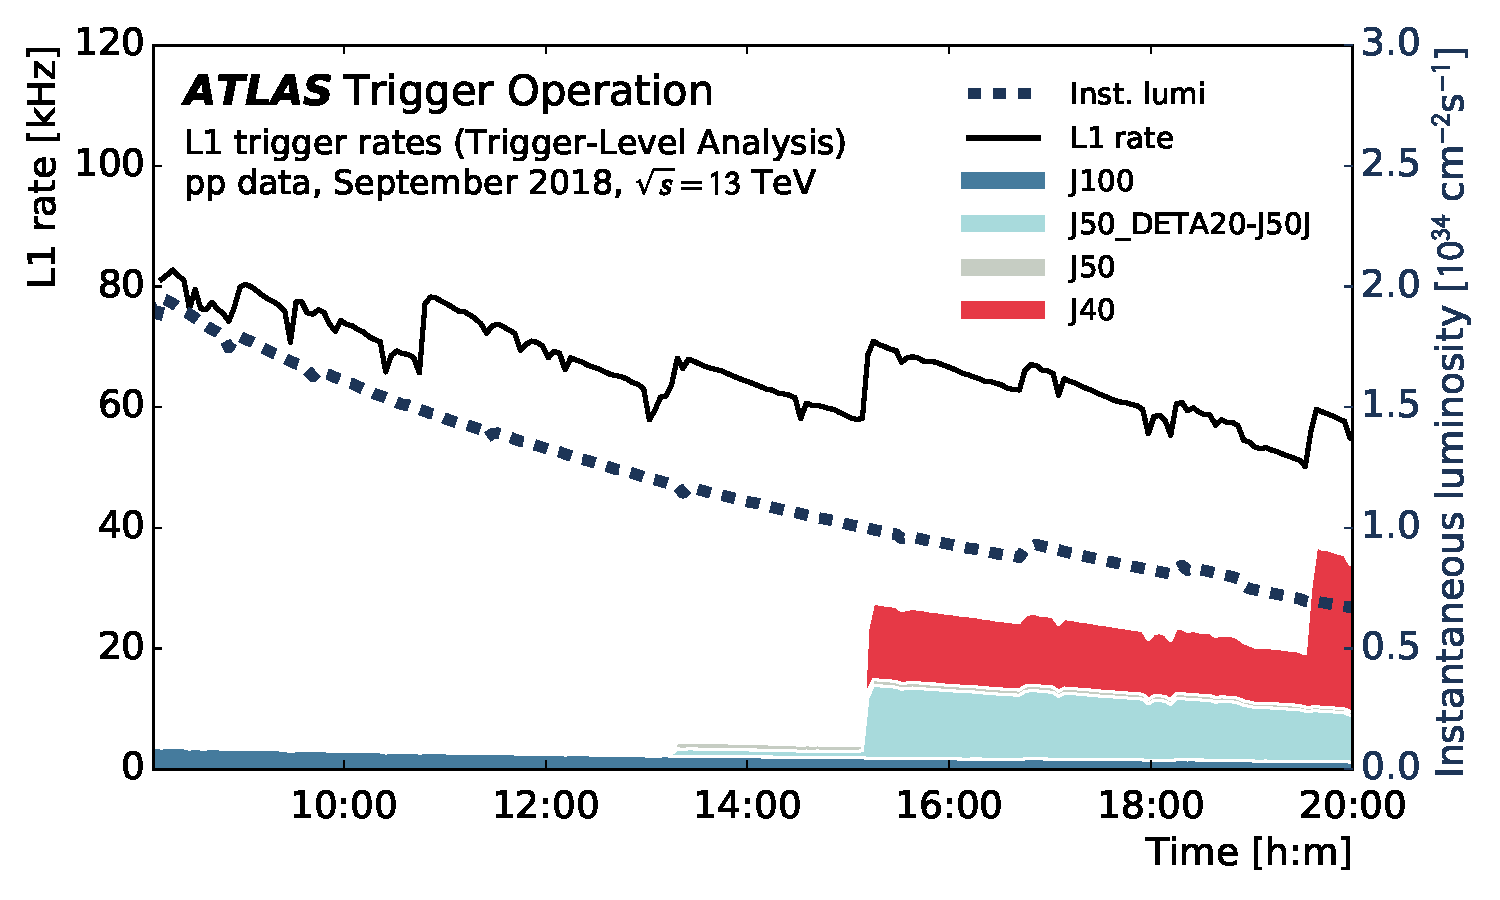
\includegraphics[width=0.48\textwidth]{figs_B2/TLAPublicWinter2019_L1Lumi.pdf}
\caption{\color{black}\label{fig:triggerLowThreshold} \small In Run-2, the underutilization of HLT resources at low LHC instantaneous luminosity allowed my team and collaborators to design TLA L1 triggers with reduced $p_\mathrm{T}$ thresholds~\cite{ToBeCited}.} %Trigger operation page
\vskip2pt
\end{center}
\end{wrapfigure}
%\vskip5pt

The outcome of this work will be technical performance publications \textbf{[12]}, and contributions to early searches and measurements. 
If the sensitivity of mediator searches in the dijet mass spectrum improves with respect to Run-2 results, we will publish dijet and dijet+ISR searches using early data.
As an example, if the LHC delivers more than $\approx$ 18/fb of low-luminosity runs, dijet searches can profit from much lower jet trigger thresholds as shown in Fig.~\ref{fig:triggerLowThreshold} and surpass sensitivity with respect to current searches\footnote{The analysis of NN/fb of low-threshold Run-2 data is undergoing as part of my VR project grant, see Funding ID in Part B1}. 

Another important component of this proposal developed in WP2 is \textbf{reproducible end-to-end analysis software for dijet and dijet+ISR DM mediator searches [12]}. 
We will use the RECAST framework to package the entire software stack used for early data analyses so that many of the steps can be executed automatically rather than manually.
Using RECAST at this early stage has three advantages. 
Firstly, it makes intermediate testing and monitoring much faster, as this code can be executed on new data and compared to already-tested data. 
Secondly, it shortens the time required to go from calibrated data to final plots and analysis results in the analysis iteration with the full LHC dataset in WP3.
Thirdly, it can be used as back-end to the REANA framework~\cite{ToBeCited}. %REANA
so that theorists and members of the DM community can test their own signals, as discussed in WP5.  

\subsubsection{Objectives of WP3}

The overall objective of WP3 is to use Run-3 LHC data recorded with the TLA technique to search for new resonances in the dijet mass spectrum, motivated by DM mediators.
In this proposal we will focus on the decays of the mediators to light quarks, but the work in WP1 also enables dedicated searches for mediators decaying preferentially to heavy quarks. 

The main innovation in this WP is the \textbf{dijet+ISR photon search using the TLA technique}, alongside the signature of a gluon ISR\textbf{[13]}. 
The two channels are complementary: the jet ISR channel is more sensitive due to higher signal rates, but selecting events using photon ISR can reach lower mediator masses. 
Both channels will be much more sensitive than current Run-2 traditional searches, since the threshold on the associated object is lowered from $\approx$ 400 GeV to $\approx$ 220 GeV and from $\approx$ 150 GeV to $\approx$ 40 GeV for jet and photon cases respectively.  
In turn, this increases the signal acceptance of more than one order of magnitude for a mediator mass of 250 GeV~\footnote{The background also increases, but since it is estimated using data-driven techniques as explained in~\ref{sec:methodologies} its increase can be managed without a significant loss in sensitivity.}, 
and it lowers the minimum mediator mass to which these searches are sensitive, as shown e.g. in Ref.~\ref{ToBeCited}.%CMS ISR TLA 
Throughout WP3, will rely on calibrations and data analysis code developed and tested in WP1 and WP2, in particular on the pile-up suppression techniques for the low-$p_{\mathrm{T}}$ jets that compose the resonance and on the RECAST implementation of the dijet+ISR signature. 
We will also maintain our involvement in the \textbf{full Run-2 + Run-3 dataset dijet TLA}, providing the WP2 RECAST implementation and working with collaborators.  
We will combine Run-2 and Run-3 results for a legacy TLA publication covering both LHC runs \textbf{[14]}. 
Dijet searches are sensitive to a variety of new physics signals (see Sec.~\ref{sub:stateOfTheArtTheory}): code and results from WP3 searches will be input to WP5 for broad dissemination. 

\subsubsection{Objectives of WP4}

%CD: I have the feeling this is a combination of objectives and methods
The objective of WP4 is to use Run-3 LHC data recorded with the TLA+PEB technique for dark QCD searches. 
The work in WP1 and WP2 on the reconstruction, calibration and performance of regional detector data will be the stepping stone for the searches for semi-visible jets and composite jets. 
In WP4, we will \textbf{extend the study of isolated object performance to busier hadronic environments}, with a focus on the identification of variables and analysis techniques that can be used to minimize the impact of pile-up and reduce SM backgrounds already at the trigger level \textbf{[15]}. 
Rejecting sufficient QCD background with a pre-selection will allow recording higher rate of TLA+PEB events with lower thresholds with respect to offline searches, with sufficient raw detector information in the region behind the jets. 
These studies will also give sufficient handles to understand the variability of QCD jets to evaluate search sensitivity and systematic uncertainties.
They will also provide input to a parallel effort funded by my VR Project Grant focused on anomaly detection techniques.  
The \textbf{search for semi-visible jets} will be performed first~\textbf{[16]}, after we have reached sufficient understanding of the hadronic jet content. 
Subsequently, we will augment the standard reconstruction techniques to correctly identify anomalous content (e.g. leptons in jets) needed for the \textbf{composite jet search}~\textbf{[17]}.

An additional advantage of the PEB+TLA data stream selected for these searches is that it enables searches for a wide variety of non-standard jet topologies (e.g. photon-jets~\cite{PhotonJets}, jets containing long-lived particles~\cite{PhotonJets}) at a later date. 
This will have an impact especially after the end of this proposal when the long LHC shutdown is foreseen before HL-LHC and data already taken will be analyzed in further detail. 

\subsubsection{Objectives of WP5}

The overall objective of WP5 is to connect the results in this proposal to the broader experimental community, with a focus on the search for DM, to maximize their impact. 
This WP naturally includes the contextualization, communication and dissemination of results, in terms of tools that can enhance the physics potential of experiments and of DM discoveries or constraints. WP5 also covers my work within synergistic initiatives involving LHC experiments and the broader DM search communities that directly benefit the objectives of WP3 and WP4, started with the Dark Matter Forum and in the context of the update of the European Strategy of Particle Physics. Collectively furthering the DM community’s understanding of the theoretical and experimental landscape for WIMP and dark QCD models will sharpen the LHC search targets. WP5 spans the entire course of this project, and has four goals. 

Firstly, we will collaborate with theory experts in Lund, Heidelberg and worldwide to \textbf{identify the most promising parameter space for the searches in WP4}, in order to develop trigger chains that can best target it~\textbf{[18]}. 
Concretely, this will take place through shared supervision of PhD students and dedicated workshops in Lund, similar to the 2019 Dark Jets workshop~\cite{ToBeCited}. %DarkDijetsWorkshop
These workshops will allow cross-talk with the community interested in comparing and contrasting regular and dark QCD, leading to concrete improvements for MC generation. 

Secondly, I will \textbf{continue co-organizing the Initiative for DM in Europe and beyond (\href{https://indico.cern.ch/e/iDMEu/}{iDMEu})}, a cross-community effort focused on DM that includes the nuclear physics, astroparticle physics and particle physics. 
This initiative has more than 200 endorsers at the time of writing, and will have its first kick-off meeting in early Summer 2020. 
It has the ambition of becoming a permanent forum so that all different communities can identify opportunities to work together and exploit synergies and complementarities. 
Practical outcomes of work within this initiative are summary plots with commonly used benchmarks that enhance the complementarity of the LHC results in WP3 and WP4 with other experiments and astrophysical observations~\textbf{[19]}. iDMEu also includes a component of communication to the general public, also part of WP5~\textbf{[20]}. 

Thirdly, we will \textbf{disseminate the technical outcomes of WP1 to other experiments at the LHC and beyond}. 
This will be achieved via technical peer-reviewed papers that include links to prototype open source software implementations as auxiliary materials and presentation in conferences. 
I have recently become part of the coordination team of the cross-experiment \href{https://hepsoftwarefoundation.org}{HEP Software Foundation} (HSF). 
With its goal of helping experiments meeting the challenges posed by new experimental programmes for HL-LHC, the HSF is an ideal platform to connect the solutions in this proposal to experimental needs~\textbf{[21]}. 
%This goal also includes concrete work on data compression with the EGO/Virgo experiment. 

The fourth goal of WP5 is to \textbf{make results and data from WP3 and WP4 as accessible as possible}, both inside and outside the ATLAS collaboration. 
We will publish the final analysis likelihoods from WP2-4 and implement the end-to-end RECAST analyses in the REANA hub~\cite{ToBeCited}, %REANA
so that they can be scrutinized and reproduced without a need to directly access ATLAS data (which will only be available in open format at a later date)~\textbf{[22]}.
These analyses will become part of a broader effort the cross-experiment \textit{Virtual DM environment} for end-to-end data analysis within the European Science Cluster of Astronomy and Particle Physics ESFRI research infrastructure (ESCAPE), which I will start leading at the beginning of 2020. 
All software implementations within this project will become part of the \href{https://projectescape.eu/services/escape-software-data-catalogue}{ESCAPE Software Catalogue}. 




